% This is samplepaper.tex, a sample chapter demonstrating the
% LLNCS macro package for Springer Computer Science proceedings;
% Version 2.20 of 2017/10/04
%
\documentclass[runningheads]{llncs}
%
\usepackage{graphicx}
% Used for displaying a sample figure. If possible, figure files should
% be included in EPS format.
%
% If you use the hyperref package, please uncomment the following line
% to display URLs in blue roman font according to Springer's eBook style:
% \renewcommand\UrlFont{\color{blue}\rmfamily}

\begin{document}
%
\title{MRI Face Detector}
%
%\titlerunning{Abbreviated paper title}
% If the paper title is too long for the running head, you can set
% an abbreviated paper title here
%
\author{%
Avinash Kori\inst{1,2}\orcidID{} %
\and Shashank Bansal\inst{2}\orcidID{} %
\and Oscar Esteban\inst{2}\orcidID{} %
\and Joe Wexler\inst{2}\orcidID{} %
\and Russell Poldrack\inst{2}\orcidID{}} %
%
\authorrunning{A. Kori et al.}
% First names are abbreviated in the running head.
% If there are more than two authors, 'et al.' is used.
%
\institute{%
Indian Institute of Technology (IIT), Madras, India
%% The email below was lncs@springer.com - I am guessing this is a placeholder email
\email{}\\
\and Dept. of Psychology, Stanford University, Stanford, USA}
%
\maketitle              % typeset the header of the contribution
%
\begin{abstract}
Image defacing is essential for anonymizing and protecting the identity of the MR brain scan. While there are a few automated tools that deface a faced image, there are currently no tools that can efficiently and accurately detect if the brain volume has been defaced. Here we introduce the MRI Face Detector tool, a framework for extracting the structural information from the brain volume and classifying if the volume has been defaced. The classifier was trained using a projection based 2.5D U-net architecture on publicly available, multi-site data volumes (N = 1236) taken from 41 different datasets. Class prediction is calculated using 3 independent models generated in a cross-validation fashion which are then merged to obtain an average confidence score for the input volume. The model obtained an accuracy of 0.948 on a held-out dataset *DATASET INFO*. Furthermore, the model architecture achieved a sensitivity and specificity of 0.945 and 0.949 respectively.

\keywords{}
\end{abstract}
%
\section{Introduction}


\newpage
\section{Materials and Methods}
\subsection{Overview}
\begin{figure}
 \centering
 \label{fig:overview}
 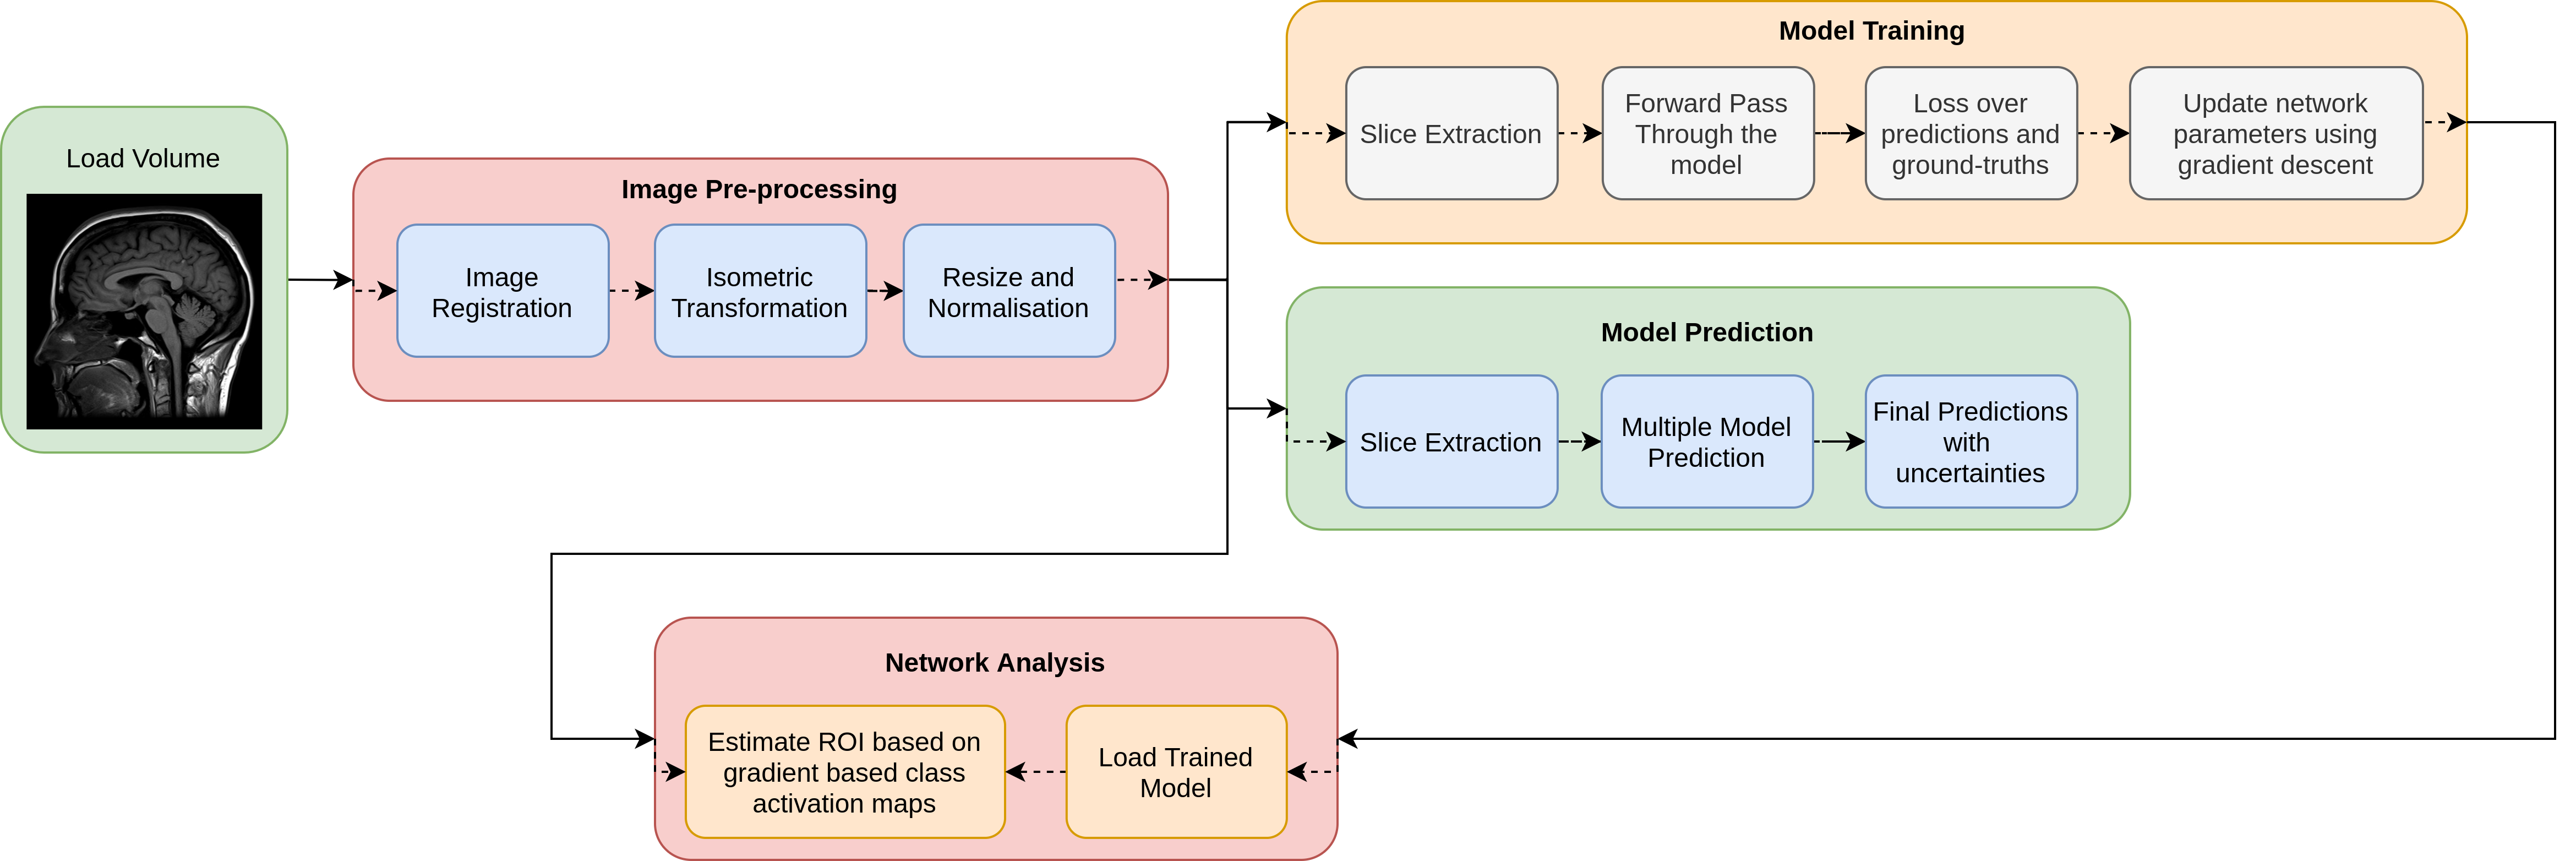
\includegraphics[width=1\textwidth]{images/overview.png}
 \caption{}
\end{figure}

Figure \ref{fig:overview}, describes the overall structure of our framework. The proposed framework detects if the given T1 weighted MR image is faced or defaced. Which in the process involves volume registration to a fixed atlas image, isotropic transformation to standardize the voxel size along all the axis, volume normalization to bound the range of input, followed by slice sampling, and prediction. We perform network analysis to qualitatively quantify the learning of the network using Gradient-based class activation maps, and also estimate uncertainties on prediction to provide confidence bounds on the prediction. 


\subsection{Data}
\begin{figure}
 \centering
 \label{fig:volumecount}
 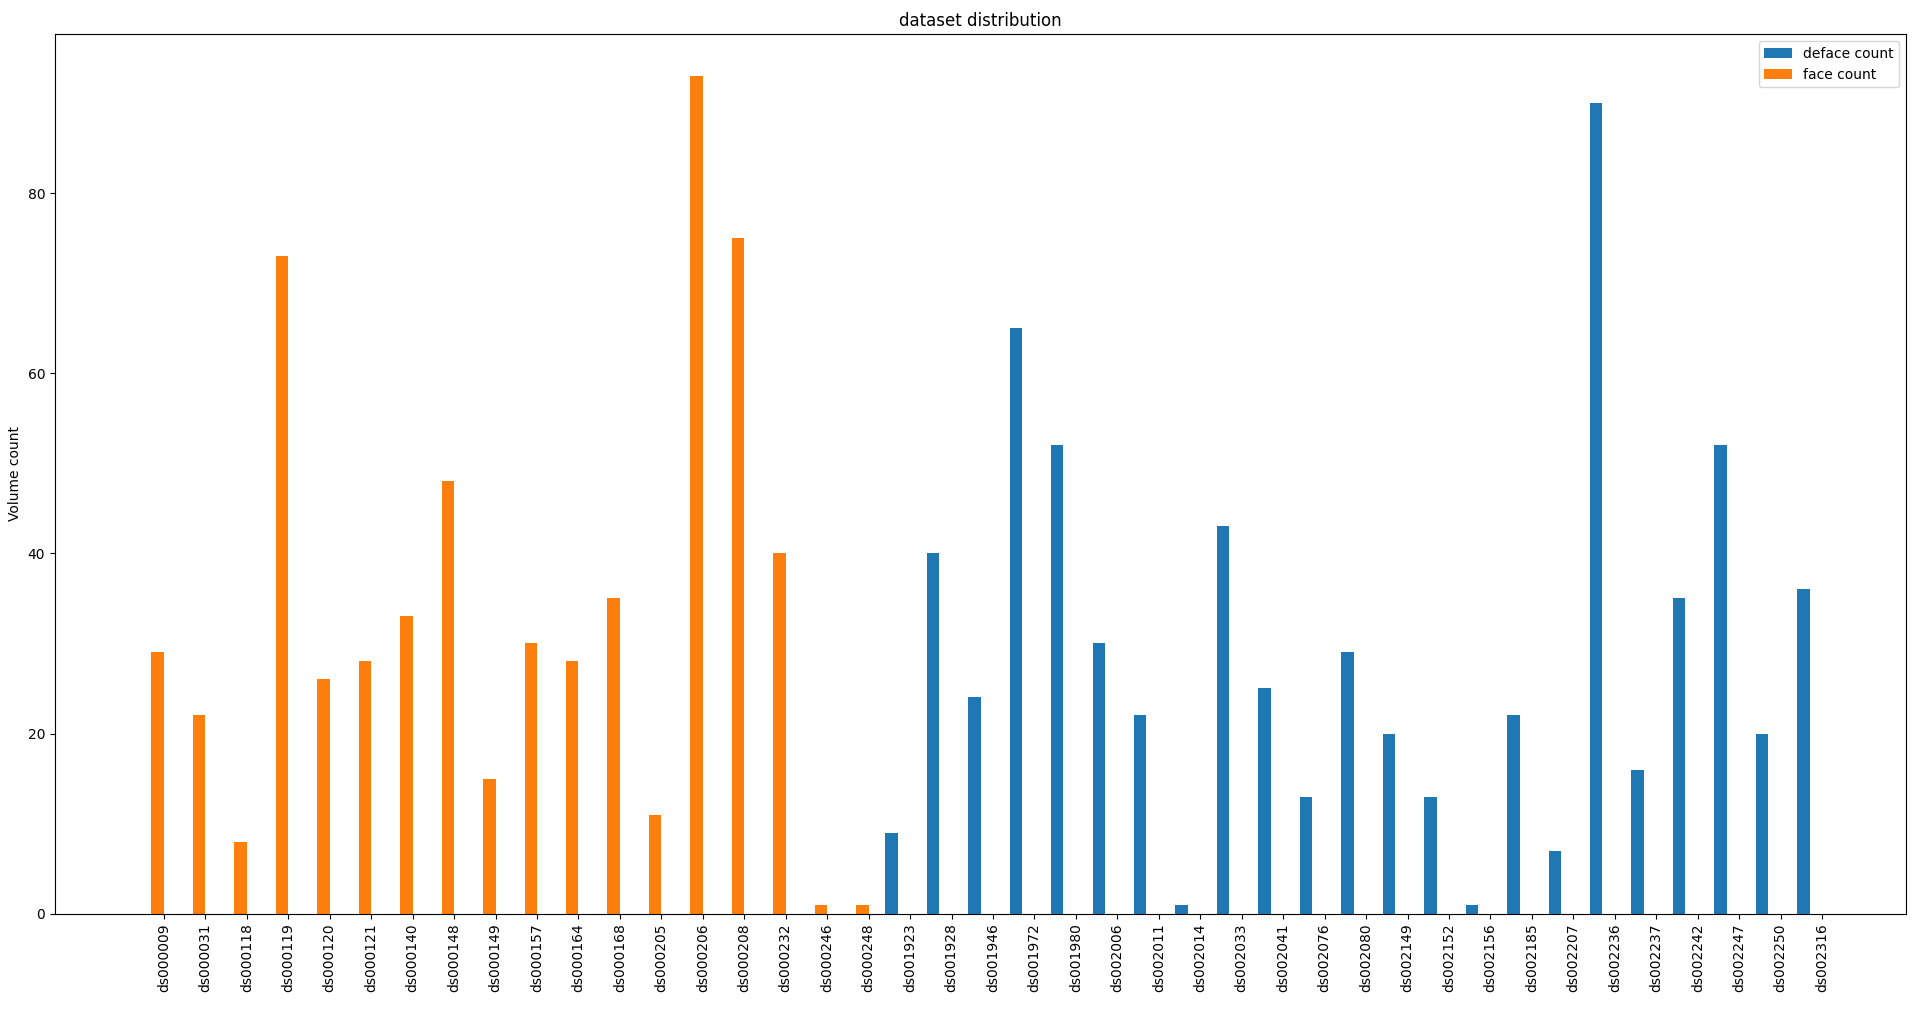
\includegraphics[width=1\textwidth]{images/volumecount.png}
 \caption{}
\end{figure}

In total, we made use of 2143 T1w volumes obtained from multiple datasets, which included 1236 training samples and 907 test samples. Each volume was assessed manually by an expert rater and classified into 4 different categories 'faced', 'defaced', 'edge-faced', and 'edge-defaced'. Figure \ref{fig:data} describes the difference between the volumes belonging to each class.

For training we considered 1236 T1w volumes which included only 'faced' and 'defaced' data, edge cases were pushed to test set. Figure \ref{fig:volumecount} describes a number of faced and defaced volumes taken from each dataset that was used in training. In total, about 596 faced volumes and 665 defaced volumes were used in training.

\begin{figure}
 \centering
 \label{fig:data}
 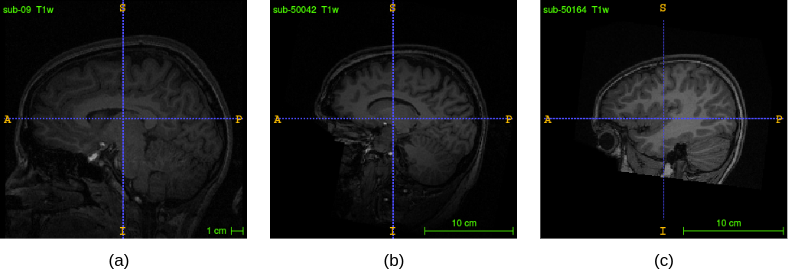
\includegraphics[width=1\textwidth]{images/data.png}
 \caption{}
\end{figure}


To investigate the robustness and generalizability of the technique we made use of the 3 fold cross-validation approach. Where each time we excluded multiple datasets from the training and added them to the validation set. Leave one site out (LoSo) as proposed in \cite{} couldn't be used because (i) We made use of a large number of datasets (41 different datasets) (ii) Most of the datasets just had faced or defaced volume which could skew the learning by adding additional bias. Table \ref{table:cvsplit} describes the split of data in each cross-validation set.  

\begin{table}[]
\centering
\label{table:cvsplit}
\begin{tabular}{|c|c|c|c|c|c|c|c|}
\hline
\multirow{}{}{} & Total & \multicolumn{2}{c|}{\begin{tabular}[c]{@{}c@{}}Cross Validation \\ Set 1\end{tabular}} & \multicolumn{2}{c|}{\begin{tabular}[c]{@{}c@{}}Cross Validation\\ Set 2\end{tabular}} & \multicolumn{2}{c|}{\begin{tabular}[c]{@{}c@{}}Cross Validation\\ Set 3\end{tabular}} \\ \cline{2-8} 
                  &       & Training                                  & Validation                                 & Training                                 & Validation                                 & Training                                 & Validation                                 \\ \hline
Faced             & 596   & 397                                       & 199                                        & 395                                      & 201                                        & 398                                      & 198                                        \\ \hline
Defaced           & 665   & 443                                       & 222                                        & 454                                      & 211                                        & 444                                      & 221                                        \\ \hline
\end{tabular}
\caption{}
\end{table}

We illustrate the generalizability of our model by illustrating its performance on completely unseen datasets, for which we again made use of multiple open neuro datasets which included 326 T1w volumes with 223 faced volumes and 103 defaced volumes. We also tested the model adaptability on different modality, for which we show the model performance on IXI dataset \cite{} which includes 581 faced T1 volumes.


\subsection{Pre-processing of Data}
In order to address the variability in acquisition of the data, every volume was registered to fixed atlas volume, to align all the axes. To address variability in intensity values volume-wise standardization was performed followed by min-max normalization to fix the range of input between (0, 1). 

\subsubsection{Registration and Isometric Transformation}
As the data was acquired from different sites which resulted in a mismatch of volume axis, which was circumvented by registering all the volumes to a standard T1w brain atlas. The energy minimization based method as proposed in \cite{} was used for affine volume registration to allign all volumes to atlas. After registration isometric transformation was applied on a volume to maintain constant voxel dimension by trilinear interpolation.

\subsubsection{Resizing and Re-normalization of Volume}
As discussed previously, since the data was obtained from multiple sources intensity range of the MRI volumes also vary. To address this issue volume wise mean subtraction and variance normalization was performed, which results in the volume with zero mean and unit standard deviation. Followed by min-max normalization step, which ensures that the range of volume is between (0,1). The equations \ref{eqn:normalization}, \ref{eqn:minmax} describes the afformentioned transformation.
\begin{equation}
 \label{eqn:normalization}
 X_{std} = \frac{X - \mu}{\sigma^2}
\end{equation}

\begin{equation}
 \label{eqn:minmax}
 X_{norm} = \frac{X_{std} - min(X_{std})}{max(X_{std}) - min(X_{std})}
\end{equation}

\subsubsection{Slice Extraction}
Since the number of data points was limited, a 2.5D convolutional neural network as proposed in \cite{} was adapted to model the conditional for face detection. In the case of training and inference, uniform random sampling was performed to sample slices from axial, coronal, and sagittal axis.

\subsection{Training Pipeline}
\subsubsection{Network Architecture}
\begin{figure}
 \centering
 \label{fig:network}
 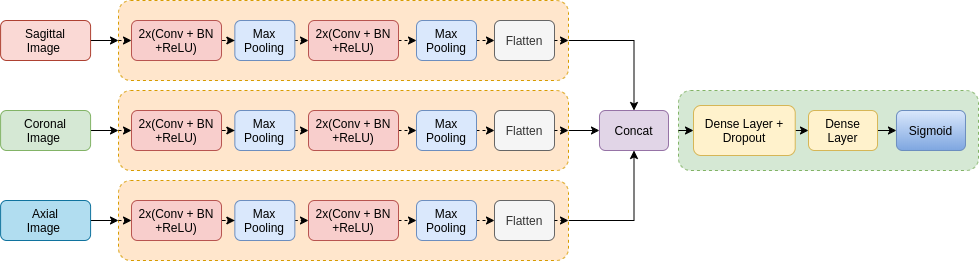
\includegraphics[width=1\textwidth]{images/network.png}
 \caption{}
\end{figure}

\subsubsection{Loss function}


\subsection{Inference Pipeline}

\subsection{Network Analysis}
\subsubsection{Uncertainty Estimation}
\subsubsection{GradCAM Analysis}


\newpage
\section{Results and Discussion}
\begin{figure}
 \centering
 \label{fig:faceCAM}
 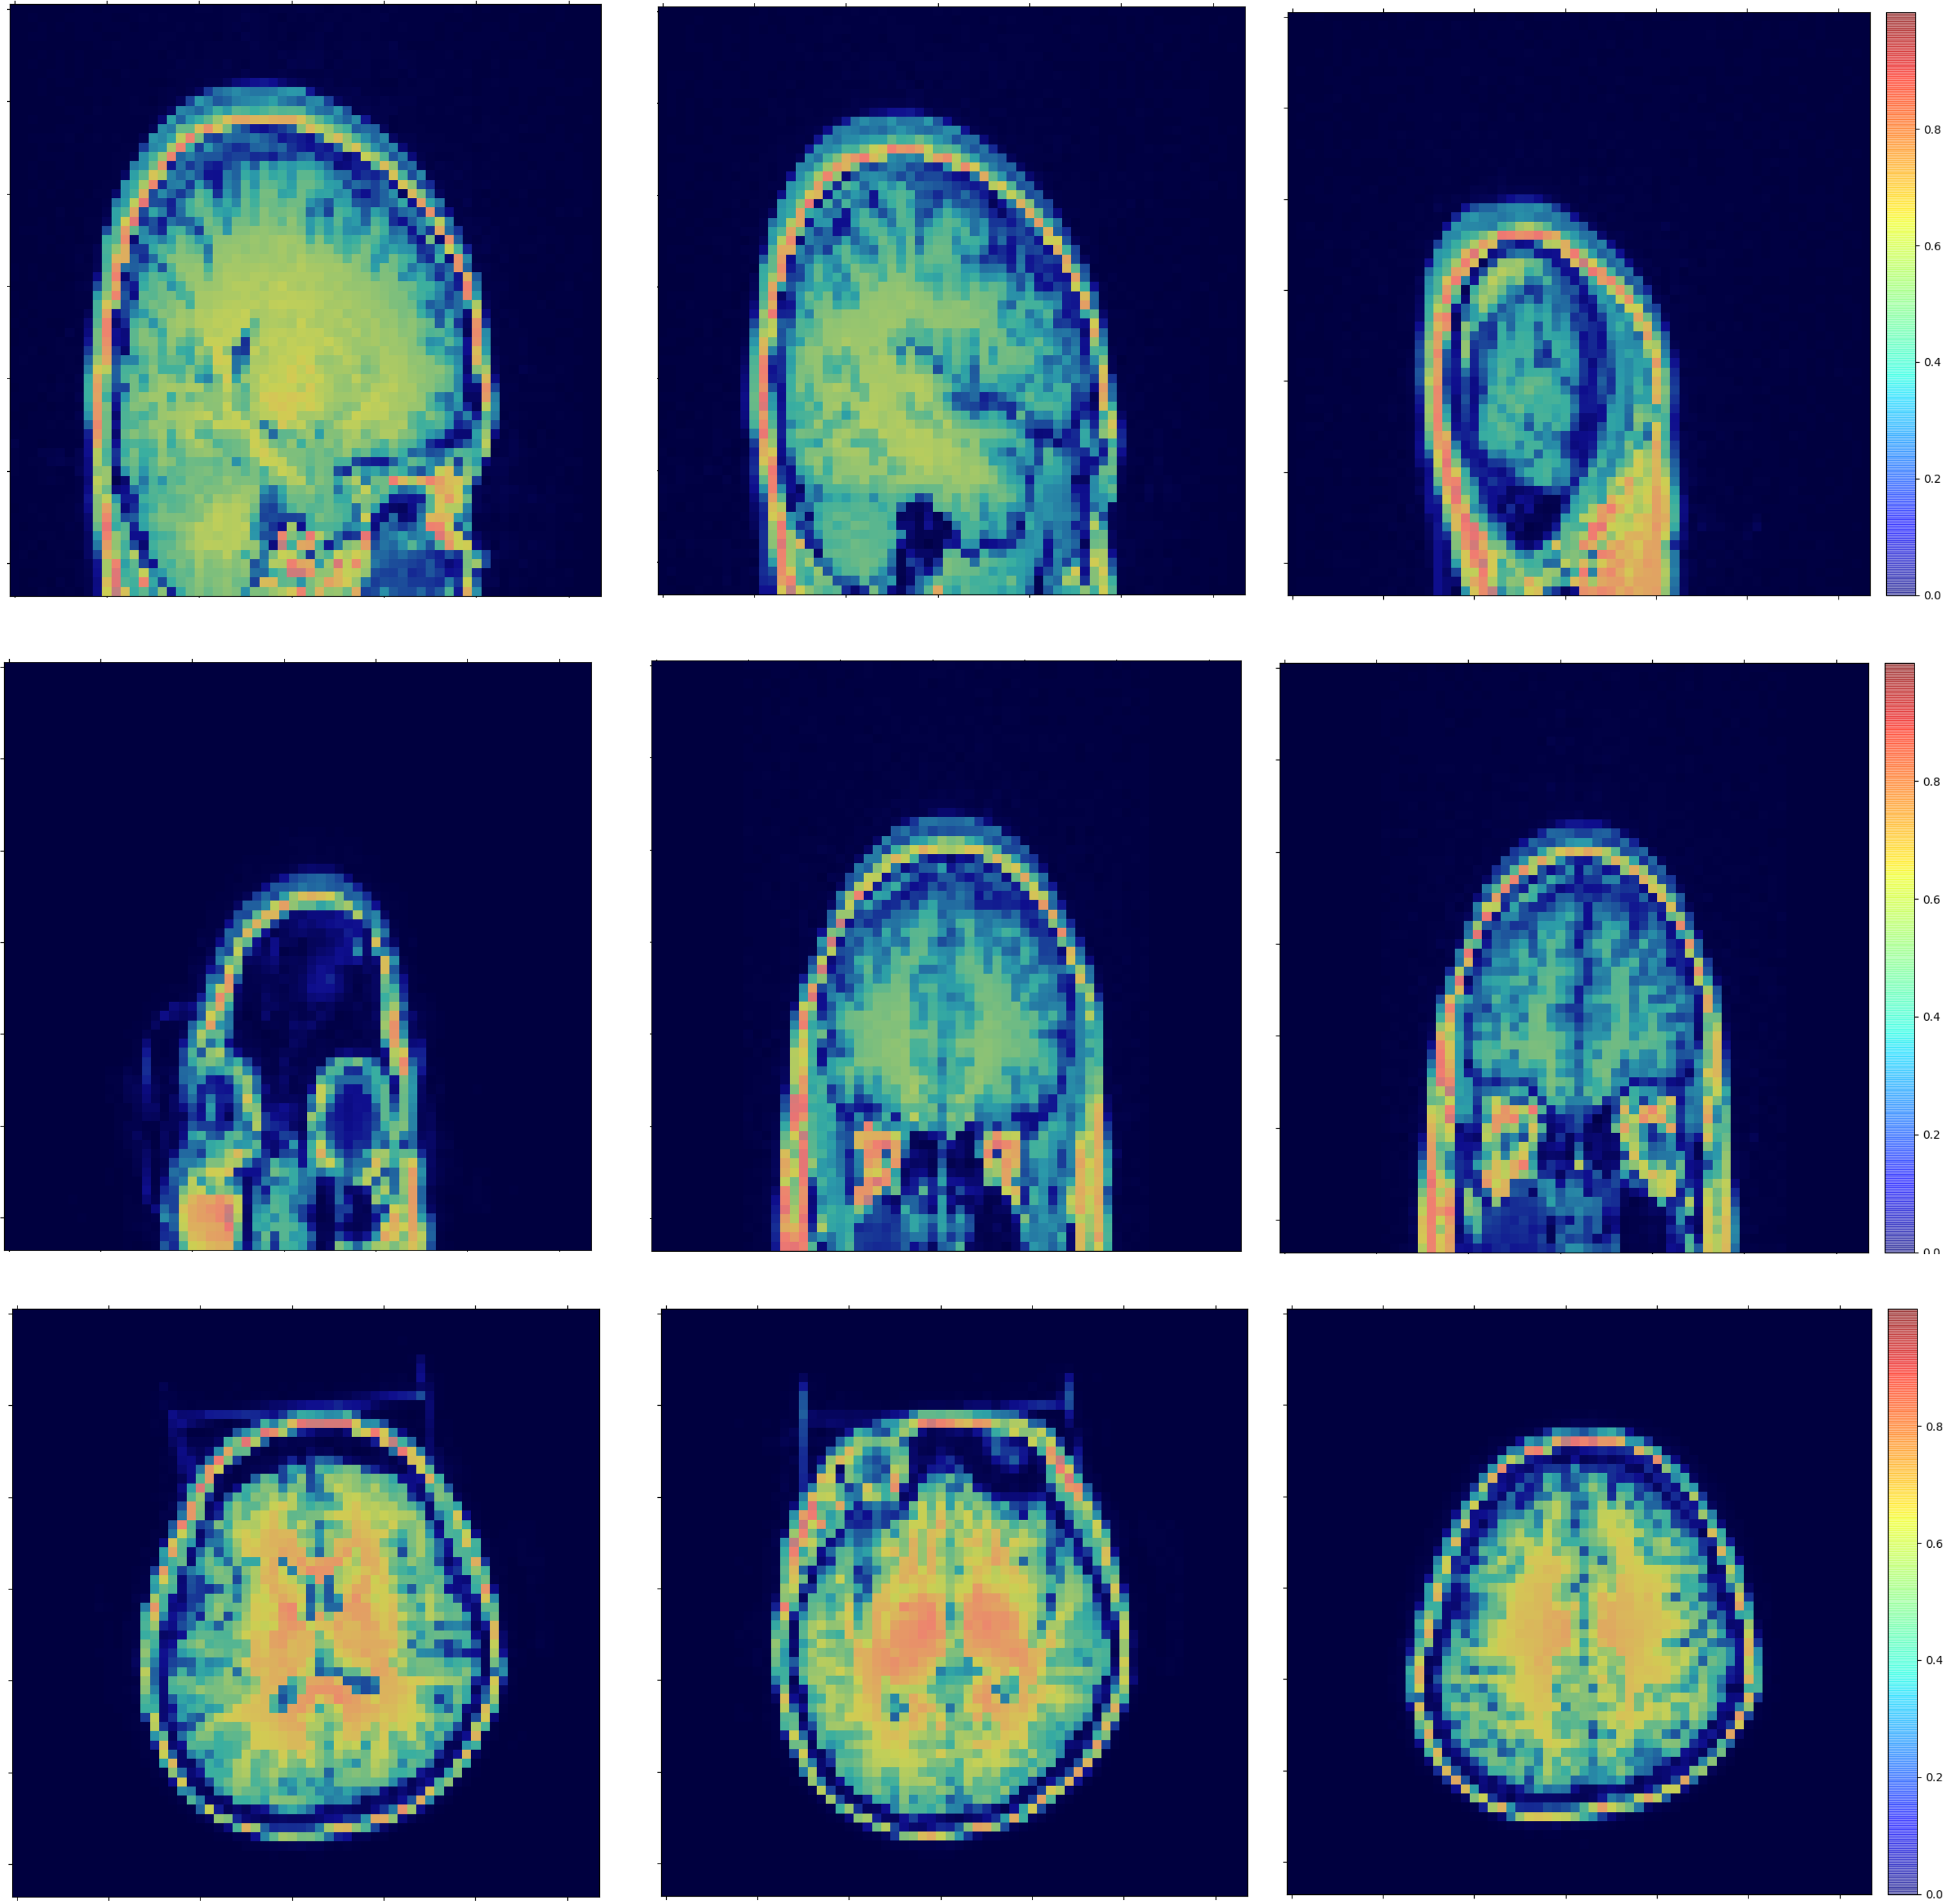
\includegraphics[width=1\textwidth]{images/faceCAM.png}
 \caption{}
\end{figure}

\begin{figure}
 \centering
 \label{fig:defaceCAM}
 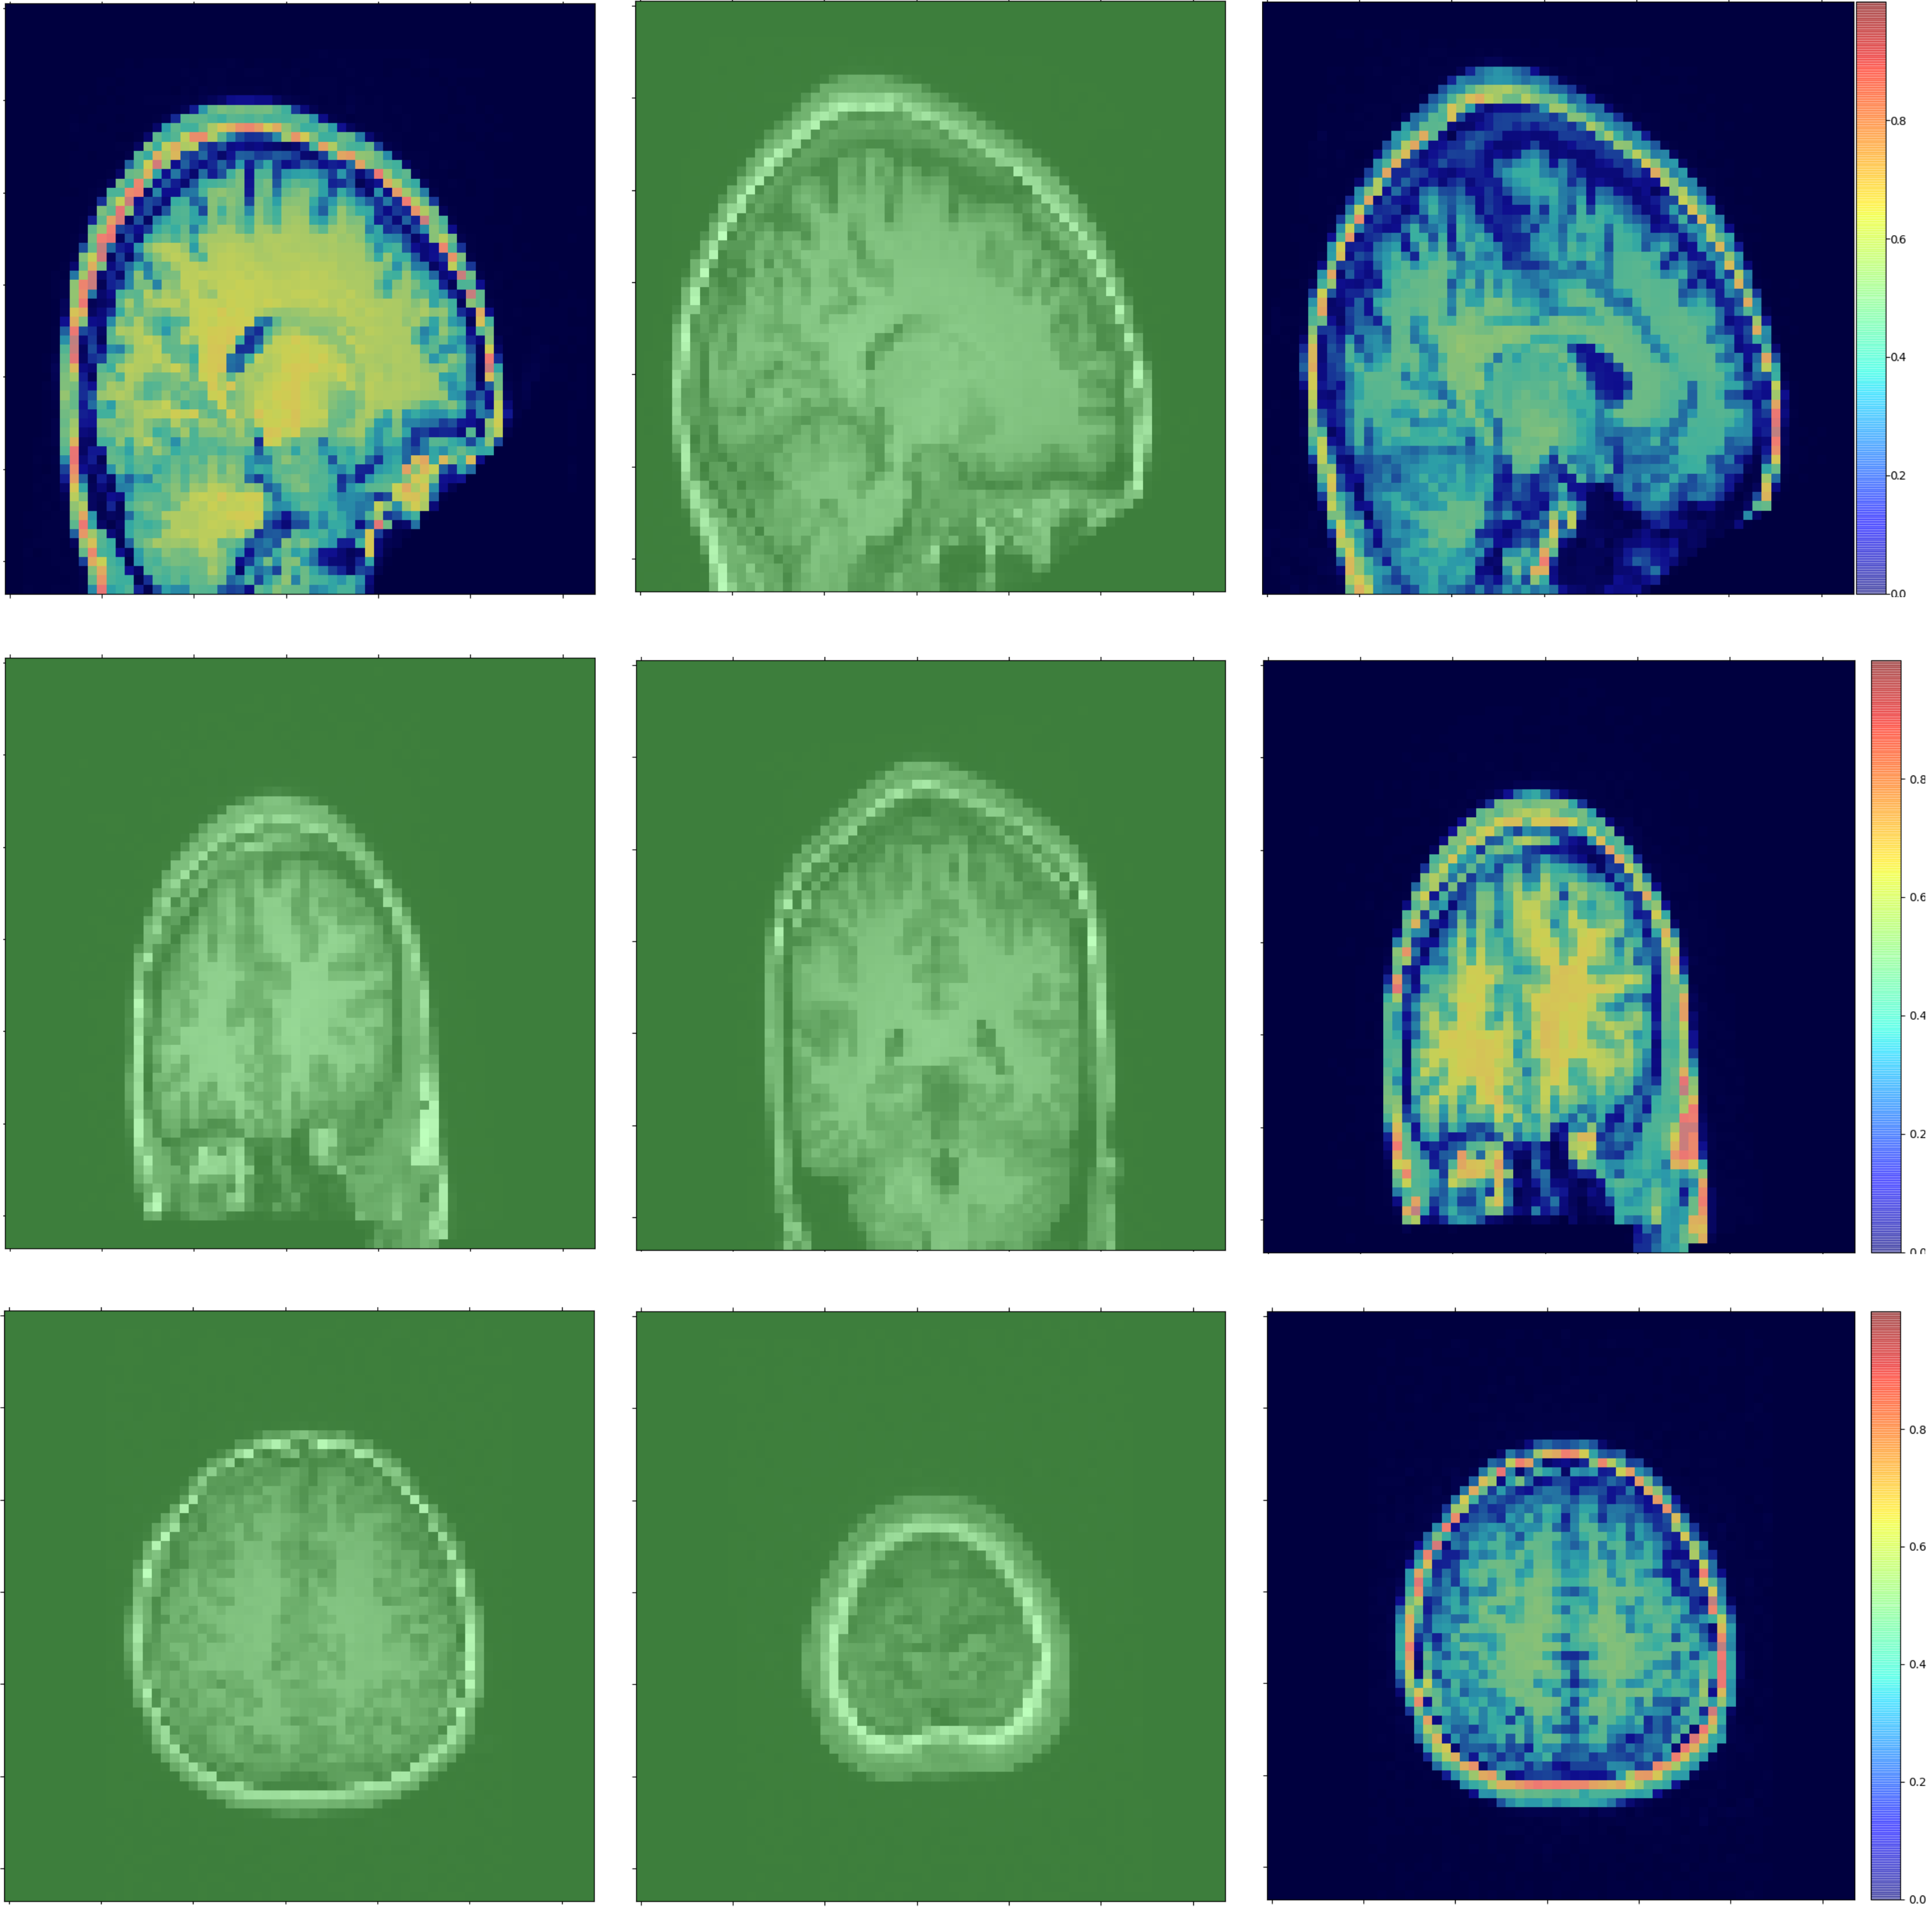
\includegraphics[width=1\textwidth]{images/defaceCAM.png}
 \caption{}
\end{figure}
\end{document}
